\section{Overview}

This chapter discusses some rules for bid changes that are not the rule based on rule-based bidding or visibility-based bidding. These rules are applied after the rule-based bidding and visibility-based bidding. The main part of this is the mismatch that we do, the capping of minimum and maximum bids and applying any filters that are required.

\section{Optimum Bid Range}

The optimum bid is the bid that is calculated by the algorithm. While calculating the bid range, we make sure that the bids are not very high compared to the optimum bid.


\subsection{\_comply\_bid\_range\_one Function}

\begin{lstlisting}[language=Python]
def _comply_bid_range_one(row):
    # ... (code omitted for brevity)
    return round(bid, 2)
\end{lstlisting}

This function complies the bid range for a single row of data. The function takes as input a Series \verb|row| which contains the data for a single row.

The function first checks if the \verb|action| value in \verb|row| is null. If it is, the function sets \verb|bid| to the \verb|sys_bid| value in \verb|row| and returns it.

The function then checks if the \verb|clicks| or \verb|impressions| value in \verb|row| is 0. If either is 0, the function sets \verb|bid| to the \verb|sys_bid| value in \verb|row| and returns it.

The function then checks if the \verb|action| value in \verb|row| is "visibility targets". If it is, the function sets \verb|bid| to the minimum of the \verb|sys_bid| value in \verb|row| and 1.4 times the \verb|mean_bid| value in \verb|row|. If \verb|action| is not "visibility targets", the function sets \verb|bid| to the minimum of the \verb|sys_bid| value in \verb|row| and 1.15 times the \verb|mean_bid| value in \verb|row|.

Finally, the function returns \verb|bid| rounded to 2 decimal places.

The figure \ref{fig:comply_bid_range_one} shows a tree diagram of the logic of the function:

\begin{figure}
    \centering
    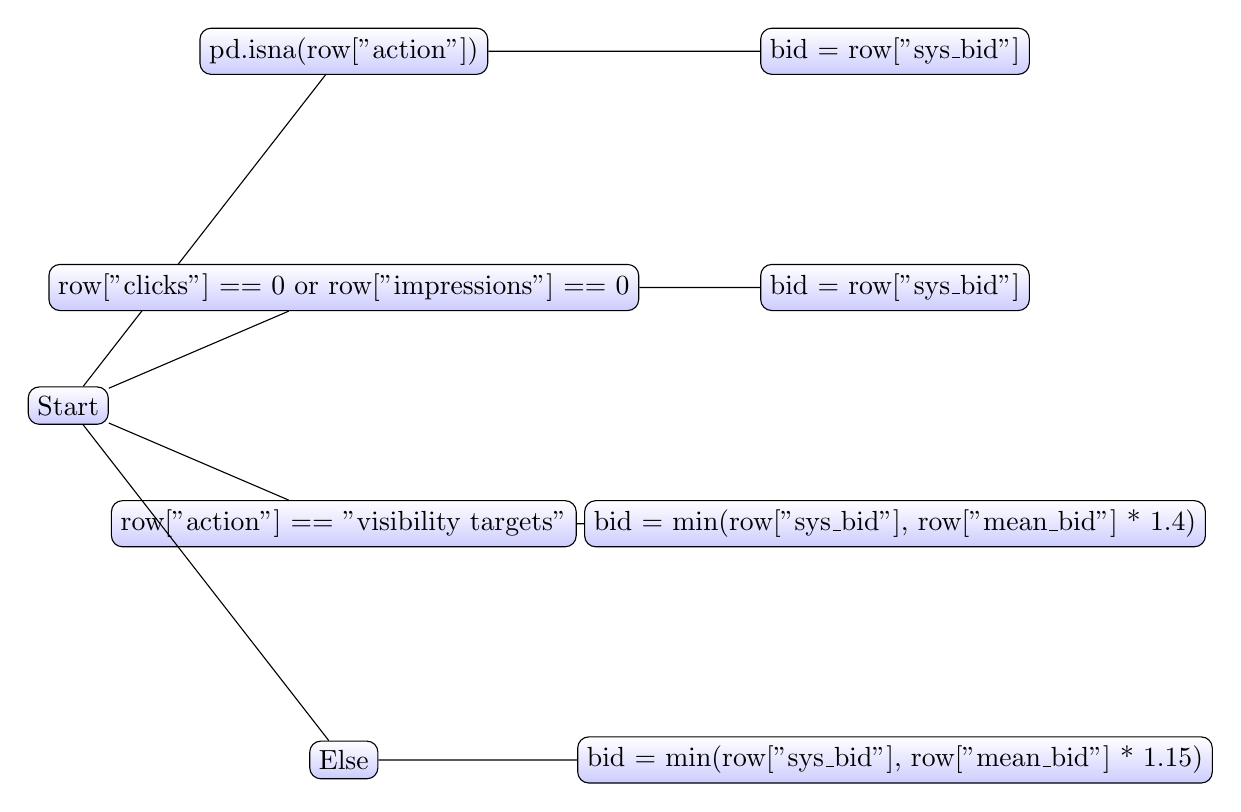
\begin{tikzpicture}[
            grow'=right,
            level 1/.style={level distance=3.5cm, sibling distance=3cm},
            level 2/.style={level distance=7cm, sibling distance=2cm},
            every node/.style = {shape=rectangle, rounded corners, draw, align=center, top color=white, bottom color=blue!20}
        ][scale=0.8]

        \node {Start}
        child { node {pd.isna(row["action"])}
                child { node {bid = row["sys\_bid"]} }
            }
        child { node {row["clicks"] == 0 or row["impressions"] == 0}
                child { node {bid = row["sys\_bid"]} }
            }
        child { node {row["action"] == "visibility targets"}
                child { node {bid = min(row["sys\_bid"], row["mean\_bid"] * 1.4)} }
            }
        child { node {Else}
                child { node {bid = min(row["sys\_bid"], row["mean\_bid"] * 1.15)} }
            };

    \end{tikzpicture}
    \caption[short]{Logic For Complying Bid}
    \label{fig:comply_bid_range_one}
\end{figure}

\subsection{set\_bid\_range Function}

\begin{lstlisting}[language=Python]
def set_bid_range(data_with_sys_bid, client_profile_id):
    # ... (code omitted for brevity)
    return data_with_sys_bid
\end{lstlisting}

This function sets the bid so that the bid complies with the bid range. The function takes as input a DataFrame \verb|data_with_sys_bid| which contains the data with system bids generated using the \verb|calculate_sys_bid| function, and a string \verb|client_profile_id| which is the client profile id.

The function first retrieves a list of unique \verb|Targeting_ID| values from \verb|data_with_sys_bid|. It then constructs a SQL query to retrieve the \verb|Targeting_ID|, \verb|client_profile_id|, \verb|mean_bid|, \verb|min_bid|, \verb|max_bid|, \verb|type| as \verb|bid_range_type|, and \verb|Date| from the \verb|max_bid_range| table where the \verb|client_profile_id| matches the input and the \verb|Date| is the maximum date for the \verb|client_profile_id| and the \verb|Targeting_ID| is in the list of unique \verb|Targeting_ID| values.

The function then runs the query and retrieves the data into a DataFrame \verb|bid_range_df|. It logs the shape of \verb|bid_range_df| and the date for \verb|bid_range_df|, and then drops the \verb|Date| column from \verb|bid_range_df|.

The function then merges \verb|data_with_sys_bid| and \verb|bid_range_df| on \verb|Targeting_ID| and \verb|client_profile_id|, and applies the \verb|_comply_bid_range_one| function to the \verb|sys_bid| column of \verb|data_with_sys_bid|.

\section{Mismatch}

Mismatch in bids is done because we do not want the same bids and/or we want to give higher bids in a group of targets based on some parameters. The following functions are used to do the mismatch.

\subsection{mismatch\_bids Function}
This is the main function to be called for mismatch.

\begin{lstlisting}[language=Python]
def mismatch_bids(
    buckets_with_bid_range,
    maximum_drop=0.4,
    \=["Targeting", "Match_Type", "campaignType"],
    order_by=["desired_rank"],
    ascending=[True],
):
    # ... (code omitted for brevity)
    return final_df
\end{lstlisting}

This function creates a mismatch of bids based on the \verb|order_by| columns when grouped on \verb|mismatch_by| columns. The bids are distributed so that the maximum bid is the max bid for the group and the minimum bid is the \verb|max bid * (1-maximum_drop)|.

The function takes as input a DataFrame \verb|buckets_with_bid_range| which contains the data with buckets and bids after \verb|set_bid_range|, a float \verb|maximum_drop| which is the maximum drop in bids, a list \verb|mismatch_by| which are the columns to mismatch by, a list \verb|order_by| which are the columns to order by, and a list \verb|ascending| which determines whether the sorting is ascending.

The function first logs the mismatch and order by columns. It then groups \verb|buckets_with_bid_range| by the \verb|mismatch_by| columns and creates a list of DataFrames \verb|groups|.

The function then iterates over each group in \verb|groups|, sorts the group by the \verb|order_by| columns, calculates the maximum bid in the group, calculates the minimum bid as the maximum bid times \verb|1 - maximum_drop|, creates a list of bids from the maximum bid to the minimum bid with the number of steps equal to the number of rows in the group, and updates the \verb|sys_bid| column of the group with the bids in the list. It then appends the group to the list \verb|mismatched_groups|.

The function then concatenates \verb|mismatched_groups| into a DataFrame \verb|final_df|. It checks if the number of rows in \verb|final_df| is not equal to the number of rows in \verb|buckets_with_bid_range|. If they are not equal, it raises a \verb|MergeNotCorrect| error.

\subsection{mismatch\_for\_pt\_visibilities Function}

\begin{lstlisting}[language=Python]
def mismatch_for_pt_visibilities(data, client_profile_id, maximum_drop=0.4):
    # ... (code omitted for brevity)
    return final_df
\end{lstlisting}

This function determines which visibilities are due to PT and mismatches them. The function takes as input a DataFrame \verb|data| which contains the data with bids, a string \verb|client_profile_id| which is the client profile id, and a float \verb|maximum_drop| which is the maximum drop in bids.

The function first constructs a SQL query to retrieve the \verb|Keyword| and count of distinct \verb|targeting_type| from the \verb|visibility_clean| and \verb|campaign_master| tables where the \verb|client_profile_id| matches the input and the date is greater than the current date minus 1.

The function then runs the query and retrieves the data into a DataFrame \verb|vis|. It then retrieves a list of \verb|Targeting| values where the count of distinct \verb|targeting_type| is greater than 1.

The function then retrieves the data in \verb|data| where the \verb|action| is "visibility" and the \verb|Targeting| is in the list of \verb|Targeting| values, and logs the number of rows in this data. It then retrieves the data in \verb|data| where the \verb|Targeting_ID| is not in the list of \verb|Targeting_ID| values in this data.

The function then checks if there is any data to mismatch. If there is, it calls the \verb|mismatch_bids| function to mismatch the bids, and concatenates the mismatched data with the other data into a DataFrame \verb|final_df|. If there is no data to mismatch, it sets \verb|final_df| to \verb|data|.

The function then checks if the number of rows in \verb|final_df| is not equal to the number of rows in \verb|data|. If they are not equal, it raises a \verb|MergeNotCorrect| error.

\subsection{mismatch\_for\_spotlight Function}

\begin{lstlisting}[language=Python]
def mismatch_for_spotlight(data, maximum_drop=0.4):
    # ... (code omitted for brevity)
    return final_df
\end{lstlisting}

This function mismatches bids for spotlight campaigns. The function takes as input a DataFrame \verb|data| which contains the data with bids, and a float \verb|maximum_drop| which is the maximum drop in bids.

The function first calls the \verb|desired_rank_for_spotlight| function to retrieve the spotlight and non-spotlight data. If there is no spotlight data, it returns \verb|data|.

The function then calls the \verb|mismatch_bids| function to mismatch the bids for the spotlight data, and concatenates the mismatched data with the non-spotlight data into a DataFrame \verb|final_df|.

The function then checks if the number of rows in \verb|final_df| is not equal to the number of rows in \verb|data|. If they are not equal, it raises a \verb|MergeNotCorrect| error.

\section{Dropping Bids}

Bids are dropped for a few reasons. These are:

\subsection{Dropping Bids Due to High PT Visibility}

We need to reduce the bids of pt targets so that we can control the visibility from kt. This is done by dropping the bids of pt targets.

\subsection*{drop\_pt\_bid Function}

\begin{lstlisting}[language=Python]
def drop_pt_bid(data, client_profile_id):
    # ... (code omitted for brevity)
    return data
\end{lstlisting}

This function drops bids on pt targets that have high \verb|tos_is|. The function takes as input a DataFrame \verb|data| which contains the data with bids, and a string \verb|client_profile_id| which is the client profile id.

The function first constructs a SQL query to retrieve the \verb|Targeting_ID| and \verb|tos_is| from the \verb|table_targeting| table where the date is the current date minus 1, the \verb|client_profile_id| matches the input, the \verb|campState| is "enabled", the \verb|adGroup state| is in ["enabled", "na"], and the \verb|AM-State| is in ["enabled", "paused"].

The function then runs the query and retrieves the data into a DataFrame \verb|tos_is_df|. It then drops duplicate rows from \verb|tos_is_df|, and merges \verb|tos_is_df| with \verb|data| on \verb|Targeting_ID|.

The function then reduces the \verb|sys_bid| of pt targets that have \verb|tos_is| less than 50 and greater than or equal to 10 by 15\%, and reduces the \verb|sys_bid| of pt targets that have \verb|tos_is| greater than or equal to 50 by 25\%.

The function then calls the \verb|_add_reason| function to add a bid change reason to \verb|data|, and returns \verb|data|.

\subsection{Dropping Bids Because of High CPC}

Keywords with high CPC have their bids reduced so that the CPC and ACOS is reduced.

\subsection*{drop\_high\_cpc\_bid Function}

\begin{lstlisting}[language=Python]
def drop_high_cpc_bid(data, performing_buckets):
    # ... (code omitted for brevity)
    return data
\end{lstlisting}

This function drops bids on targets that have high cpc. The function takes as input a DataFrame \verb|data| which contains the data with bids, and a list \verb|performing_buckets| which are the performing buckets.

The function first creates a mask where the \verb|cpc| is greater than 1.5 times the \verb|desired_cpc|, the \verb|acos| is greater than 1.2 times the \verb|target_acos|, the \verb|sys_bid| is greater than 0.8 times the \verb|last_bid|, and the \verb|bucket| is not in \verb|performing_buckets|.

The function then logs the number of rows to drop bids due to high CPC, and reduces the \verb|sys_bid| of the rows where the mask is True by 20%.

The function then calls the \verb|_add_reason| function to add a bid change reason to \verb|data|, and returns \verb|data|.